\documentclass[a4paper,twoside]{article}
\usepackage[T1]{fontenc}
\usepackage[bahasa]{babel}
\usepackage{graphicx}
\usepackage{graphics}
\usepackage{float}
\usepackage[cm]{fullpage}
\pagestyle{myheadings}
\usepackage{etoolbox}
\usepackage{setspace} 
\usepackage{lipsum} 
\usepackage{caption}
\usepackage{makecell}
\setlength{\headsep}{30pt}
\usepackage[inner=2cm,outer=2.5cm,top=2.5cm,bottom=2cm]{geometry} %margin
% \pagestyle{empty}

\makeatletter
\renewcommand{\@maketitle} {\begin{center} {\LARGE \textbf{ \textsc{\@title}} \par} \bigskip {\large \textbf{\textsc{\@author}} }\end{center} }
\renewcommand{\thispagestyle}[1]{}
\markright{\textbf{\textsc{AIF401/AIF402 \textemdash Rencana Kerja Skripsi \textemdash Sem. Ganjil 2017/2018}}}

\onehalfspacing

\hyphenation{cal-cu-do-ku}
 
\begin{document}

\title{\@judultopik}
\author{\nama \textendash \@npm} 

%tulis nama dan NPM anda di sini:
\newcommand{\nama}{Michael Adrian}
\newcommand{\@npm}{2013730039}
\newcommand{\@judultopik}{Perbandingan Algoritma Backtracking dengan Algoritma Hybrid Genetic untuk Menyelesaikan Permainan Calcudoku} % Judul/topik anda
\newcommand{\jumpemb}{1} % Jumlah pembimbing, 1 atau 2
\newcommand{\tanggal}{12/09/2017}

% Dokumen hasil template ini harus dicetak bolak-balik !!!!

\maketitle

\pagenumbering{arabic}

\section{Deskripsi}

Calcudoku, atau dikenal juga sebagai KenKen, KenDoku, atau Mathdoku, adalah sebuah permainan teka-teki (\textit{puzzle}) angka yang jawabannya memerlukan perpaduan dari logika dan kemampuan aritmatika yang sederhana. Teka-teki ini mirip dengan Sudoku. Persamaannya, tujuan dari teka-teki ini adalah mengisi setiap sel (\textit{cell}) dalam jaring (\textit{grid}) dengan angka 1 sampai \begin{math}n\end{math} tanpa pengulangan angka dalam setiap kolomnya dan barisnya untuk jaring berukuran \begin{math}n \times n\end{math}, dengan \begin{math}n\end{math} adalah ukuran jaring. Tidak ada angka yang boleh muncul lebih dari sekali dalam setiap baris atau kolom jaring. Perbedaannya, jika pada Sudoku jaring berukuran \begin{math}n \times n\end{math} dibagi menjadi \begin{math}n\end{math} kandang (\textit{cage}) dengan setiap kandang terdiri atas \begin{math}n\end{math} sel, pada Calcudoku jaring dibagi menjadi sejumlah kandang yang jumlah selnya bervariasi. Setiap kandang dibatasi oleh garis yang lebih tebal daripada garis pembatas antar sel. Angka-angka dalam satu kandang yang sama harus menghasilkan angka tujuan yang telah ditentukan jika dihitung menggunakan operasi matematika yang telah ditentukan (penjumlahan, pengurangan, perkalian, atau pembagian). Angka-angka dalam satu kandang juga boleh berulang, selama pengulangan tidak terjadi dalam satu kolom atau baris yang sama. Jika kandang hanya berisi satu sel, maka satu-satunya kemungkinan jawaban untuk sel tersebut adalah angka tujuan dari kandang tersebut. Angka tujuan dan operasi matematika dituliskan di sudut kiri atas kandang. Pada awalnya, setiap sel dalam setiap kandang dalam teka-teki ini kosong. \cite{Fahda, JohannaLukasSaputra}


\begin{figure}
\centering
\captionsetup{justification=centering}
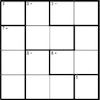
\includegraphics[scale=1]{Calcudoku1}
\caption{Contoh permainan teka-teki Calcudoku yang belum terselesaikan}
\label{fig:calcudoku1}
\end{figure}

\begin{figure}
\centering
\captionsetup{justification=centering}
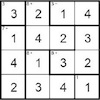
\includegraphics[scale=1]{Calcudoku2}
\caption{Contoh permainan teka-teki Calcudoku yang sudah terselesaikan}
\label{fig:calcudoku2}
\end{figure}

Calcudoku dapat diselesaikan menggunakan beberapa algoritma. Skripsi ini membahas tentang penyelesaian Calcudoku menggunakan algoritma \textit{backtracking} dan algoritma \textit{hybrid genetic}, dan perbandingan performansi \textit{performance} antara kedua algoritma tersebut.

Algoritma \textit{backtracking} adalah sebuah algoritma umum yang mencari solusi dengan mencoba salah satu dari beberapa pilihan, jika pilihan yang dipilih ternyata salah, komputasi dimulai lagi pada titik pilihan dan mencoba pilihan lainnya. Untuk bisa melacak kembali langkah-langkah yang telah dipilih, maka algoritma harus secara eksplisit menyimpan jejak dari setiap langkah yang sudah pernah dipilih, atau menggunakan rekursi (\textit{recursion}). Rekursi dipilih karena jauh lebih mudah daripada harus menyimpan jejak setiap langkah yang pernah dipilih, hal ini menyebabkan algoritma ini hampir selalu berbasis DFS (\textit{Depth First Search}). \cite{Fahda} 

Algoritma \textit{hybrid genetic} adalah gabungan antara algoritma genetik dan algoritma-algoritma lainnya. Dalam kasus ini, algoritma genetik digabungkan dengan algoritma \textit{rule based}. Algoritma genetik adalah salah satu teknik heuristik \textit{Generate and Test} yang terinspirasi oleh sistem seleksi alam. Algoritma ini adalah perpaduan dari bidang biologi dan ilmu komputer. Algoritma ini memanipulasi informasi, biasanya disebut sebagai kromosom. Kromosom ini menyandikan (meng-\textit{encode}) kemungkinan jawaban untuk sebuah masalah yang diberikan. Kromosom dievaluasi dan diberi nilai kelayakan (\textit{fitness value}) berdasarkan seberapa baikkah kromosom dalam menyelesaikan masalah yang diberikan berdasarkan kriteria yang ditentukan oleh pembuat program. Nilai kelayakan ini digunakan sebagai probabilitas kebertahanan hidup kromosom dalam satu siklus reproduksi. Kromosom baru (kromosom anak, \textit{child chromosome}) diproduksi dengan menggabungkan dua (atau lebih) kromosom orang tua (\textit{parent chromosome}). Algoritma \textit{rule based} adalah sebuah algoritma berbasis aturan logika untuk menyelesaikan permainan teka-teki Sudoku dan variasinya, termasuk Calcudoku. Beberapa aturan logika yang digunakan dalam algoritma ini adalah \textit{single square rule}, \textit{naked subset rule}, \textit{hidden single rule}, \textit{evil twin rule}, \textit{killer combination}, dan \textit{X-wing}. \cite{JohannaLukasSaputra}

\section{Rumusan Masalah}

Berdasarkan deskripsi yang telah diuraikan di atas, dapat dirumuskan permasalahan sebagai berikut:
\begin{enumerate}
\item Bagaimana cara mengimplementasikan perangkat lunak (\textit{software}) permainan teka-teki Calcudoku?
\item Bagaimana cara mengimplementasikan algoritma \textit{backtracking} untuk menyelesaikan Calcudoku?
\item Bagaimana cara mengimplementasikan algoritma \textit{hybrid genetic} untuk menyelesaikan Calcudoku?
\item Bagaimana perbandingan performansi algoritma \textit{backtracking} dengan algoritma \textit{hybrid genetic} dalam menyelesaikan Calcudoku?
\end{enumerate}

\section{Tujuan}

Berdasarkan rumusan masalah yang telah dirumuskan, maka tujuan dari pembuatan skripsi ini adalah:
\begin{enumerate}
\item Membuat perangkat lunak permainan teka-teki Calcudoku.
\item Membuat \textit{solver} untuk Calcudoku menggunakan algoritma \textit{backtracking}.
\item Membuat \textit{solver} untuk Calcudoku menggunakan algoritma \textit{hybrid genetic}.
\item Membandingkan performansi algoritma \textit{backtracking} dengan algoritma \textit{hybrid genetic} dalam menyelesaikan Calcudoku.
\end{enumerate}

\section{Deskripsi Perangkat Lunak}

Perangkat lunak akhir yang akan dibuat memiliki fitur minimal sebagai berikut:
\begin{itemize}
	\item Pengguna dapat menyelesaikan permainan teka-teki Calcudoku dengan usahanya sendiri.
	\item Pengguna dapat menggunakan algoritma \textit{backtracking} untuk menyelesaikan permainan teka-teki Calcudoku.
	\item Pengguna dapat menggunakan algoritma \textit{hybrid genetic} untuk menyelesaikan permainan teka-teki Calcudoku.
\end{itemize}

\section{Detail Pengerjaan Skripsi}

Langkah-langkah yang akan dilakukan dalam pembuatan skripsi ini adalah:
\begin{enumerate}
\item Melakukan studi literatur tentang permainan teka-teki Calcudoku.
\item Melakukan studi literatur tentang algoritma \textit{backtracking}.
\item Melakukan studi literatur tentang algoritma \textit{rule based} dan algoritma genetik.
\item Melakukan analisis dan menentukan fitur-fitur yang diperlukan dalam perangkat lunak permainan teka-teki Calcudoku.
\item Membuat perangkat lunak Calcudoku dengan fitur-fitur yang telah ditentukan. 
\item Mengimplementasikan algoritma \textit{backtracking} untuk Calcudoku.
\item Mengimplementasikan algoritma \textit{hybrid genetic} untuk Calcudoku.
\item Melakukan pengujian terhadap perangkat lunak Calcudoku yang telah dibuat, yaitu membandingkan performansi algoritma \textit{backtracking} dengan algoritma \textit{hybrid genetic} dalam menyelesaikan Calcudoku.
\item Membuat kesimpulan berdasarkan hasil pengujian perangkat lunak yang telah dibuat.
\item Menulis dokumen skripsi.
\end{enumerate}

\section{Rencana Kerja}

\begin{center}
  \begin{tabular}{ | c | c | c | c | l |}
    \hline
    1* & 2*(\%) & 3*(\%) & 4*(\%) & 5* \\ \hline \hline
    1 & 10 & 10 & 0 &  \footnotesize Sudah diselesaikan di Skripsi 1 \\ \hline
    2 & 10 & 10 & 0 &  \footnotesize Sudah diselesaikan di Skripsi 1 \\ \hline
    3 & 10 & 10 & 0 &  \footnotesize Sudah diselesaikan di Skripsi 1 \\ \hline
    4 & 5 & 5 & 0 & \footnotesize \makecell[l]{Sudah diselesaikan di S2 pengambilan kedua sebelum mengumpulkan rencana kerja} \\ \hline
    5 & 10 & 0 & 10 & \footnotesize \makecell[l]{Sudah diselesaikan di S2 pengambilan kedua sebelum mengumpulkan rencana kerja} \\ \hline
    6 & 15 & 0 & 15 &  \footnotesize Sudah diselesaikan di Skripsi 2 pengambilan pertama \\ \hline
    7 & 15 & 0 & 15 &  \footnotesize Sudah diselesaikan di Skripsi 2 pengambilan pertama \\ \hline
    8 & 5 & 0 & 5 & \\ \hline
    9 & 5 & 0 & 5 & \\ \hline
    10 & 15 & 5 & 10 & {\footnotesize Pendahuluan, Dasar Teori, dan Analisis di S1} \\ \hline
    Total & 100 & 40 & 60 & \\ \hline
	\end{tabular}
\end{center}

Keterangan (*)\\
1 : Bagian pengerjaan Skripsi (nomor disesuaikan dengan detail pengerjaan di bagian 5)\\
2 : Persentase total \\
3 : Persentase yang akan diselesaikan di Skripsi 1 \\
4 : Persentase yang akan diselesaikan di Skripsi 2 \\
5 : Penjelasan singkat apa yang dilakukan di S1 (Skripsi 1) atau S2 (skripsi 2)

\begin{thebibliography}{9}

\bibitem{Fahda}
  Asanilta Fahda,
  \emph{KenKen Puzzle Solver using Backtracking Algorithm},
  Makalah IF2211 Strategi Algoritma - Semester II Tahun 2014/2015,
  Program Studi Teknik Informatika, Sekolah Teknik Elektro dan Informatika, Institut Teknologi Bandung
  2015.
  
\bibitem{JohannaLukasSaputra}
  Olivia Johanna, Samuel Lukas, Kie Van Ivanky Saputra,
  \emph{Solving and Modeling Ken-ken Puzzle by Using Hybrid Genetics Algorithm},
  1st International Conference on Engineering and Technology Development (ICETD 2012),
  Faculty of Engineering and Faculty of Computer Science, Bandar Lampung University,
  2012.
  
\end{thebibliography}

\vspace{1cm}
\centering Bandung, \tanggal\\
\vspace{2cm} \nama \\ 
\vspace{1cm}

Menyetujui, \\
\ifdefstring{\jumpemb}{2}{
\vspace{1.5cm}
\begin{centering} Menyetujui,\\ \end{centering} \vspace{0.75cm}
\begin{minipage}[b]{0.45\linewidth}
% \centering Bandung, \makebox[0.5cm]{\hrulefill}/\makebox[0.5cm]{\hrulefill}/2013 \\
\vspace{2cm} Nama: \makebox[3cm]{\hrulefill}\\ Pembimbing Utama
\end{minipage} \hspace{0.5cm}
\begin{minipage}[b]{0.45\linewidth}
% \centering Bandung, \makebox[0.5cm]{\hrulefill}/\makebox[0.5cm]{\hrulefill}/2013\\
\vspace{2cm} Nama: \makebox[3cm]{\hrulefill}\\ Pembimbing Pendamping
\end{minipage}
\vspace{0.5cm}
}{
% \centering Bandung, \makebox[0.5cm]{\hrulefill}/\makebox[0.5cm]{\hrulefill}/2013\\
\vspace{2cm} Nama: \makebox[3cm]{\hrulefill}\\ Pembimbing Tunggal
}

\end{document}

